\documentclass[12pt]{article}
\usepackage{graphicx}
\usepackage{hyperref}
\usepackage{enumitem}
\usepackage[T1]{fontenc}
\usepackage[brazilian]{babel}
\usepackage[left=1.06cm,top=1.7cm,right=1.06cm,bottom=0.49cm]{geometry}
\usepackage{amssymb}
\usepackage{amsmath}
\usepackage[utf8]{inputenc}
\usepackage{xcolor}
\usepackage{listings}
\setlength{\parindent}{0pt}

\lstset{
  language=Python,
  basicstyle=\ttfamily\small,
  keywordstyle=\color{blue},
  commentstyle=\color{gray}\itshape,
  stringstyle=\color{red!60!black},
  numbers=left,
  numberstyle=\tiny\color{gray},
  frame=single,
  breaklines=true,
  showstringspaces=false,
  tabsize=4,
  literate={á}{{\'a}}1 {ã}{{\~a}}1 {é}{{\'e}}1 {ê}{{\^e}}1 {í}{{\'i}}1
           {ó}{{\'o}}1 {õ}{{\~o}}1 {ú}{{\'u}}1 {ç}{{\c c}}1
}

\begin{document}
    \begin{center}
    \Large\MakeUppercase{\textbf{Exercício Programa Cálculo Numérico}}\\
    João Pedro Kuhn \& Matheus da Cunha \\
    \href{https://github.com/matheusdacunha70/ExercicioCalculoNumerico}{\textbf{\textcolor{blue}{Repositório Github}}} \\
    Disciplina: Cálculo Numérico em Computadores (INE-5202) \\
    Docente:Priscila Cardoso Calegari \\
    \noindent\rule{\textwidth}{3pt}
\end{center}
    \section{Introdução}
\textbf{Objetivos:}
\begin{itemize}
    \item Implementar os métodos de Newton, Newton Modificado e Newton Discreto.
    \item Analisar as regiões de convergência em sistemas de equações não lineares.
\end{itemize}
\vspace{5pt}
Seja
$F:\mathbb{R}^2 \to \mathbb{R}^2$ e $F(\mathbf{x}) = \mathbf{0}$ 
o sistema não linear a ser analisado.
Para cada solução 
$(x_r^*, y_r^*)$, com $r = 1, 2, \ldots, L$,
desse sistema, associamos uma cor diferente 
$C_r$ 
e seja 
$C_0$ 
uma cor distinta de todas as outras.

Seja 
$k_{\max}$ 
o número máximo de iterações permitidas pelo método de Newton e
$\epsilon > 0$ 
uma tolerância.

Considere uma região do plano discreta,
$T = \{(x_i, y_j) \mid i, j = 0, 1, \ldots, N\}$.
Para cada 
$(x_i, y_j) \in T$ 
vamos aplicar o método de Newton, a partir dessa aproximação inicial 
$\mathbf{x}^{(0)} = (x_i, y_j)$. 
Vamos definir uma função 
$C(x_i, y_j) = C_r$ se $\left\| (x^{(k)}, y^{(k)}) - (x_r^*, y_r^*) \right\| < \epsilon$
, sendo $r = 1, ... L$ a quantidade de soluções do sistema, e $C(x_i, y_j) = C_0$  caso contrário. Como resultado teremos uma aproximação da região de convergência em $T$ .
Este primeiro mapa ilustra para onde a solução aproximada convergiu.
Podemos também construir um segundo mapa de convergência que vai ilustrar como a sequência convergiu.
Nesse caso, a cor associada a cada $x^{(0)} = (x_i, y_j)$ aproximação inicial, está relacionada ao número de iterações
realizadas. Assim, vamos definir a função $M(x_i, y_j) = C_k$, sendo $C_k = 1, ..., k_{max}$ o número de iterações, e $C(x_i, y_j) = C_0$, caso contrário.

    \section{Sistemas}
Para esse trabalho teremos dois sistemas distintos a serem aproximados pelo Método de Newton, Newton Modificado e Newton Discreto para sistemas não lineares, sendo eles:

\begin{equation}
    F_{1}(x,y) =
  \begin{cases}
    x^3 - 3xy^2 - 1 = 0 \\
    \hspace{7.5mm}3x^2y - y^3 = 0
  \end{cases}
\end{equation}

Com as seguintes soluções exatas do sistema:

$$
    (x^*_{1},y^*_{1}) = (1,0) 
$$
$$
    (x^*_{2},y^*_{2}) = (-\frac{1}{2},-\frac{\sqrt3}{2}), 
$$
$$
    (x^*_{3},y^*_{3}) = (-\frac{1}{2},\frac{\sqrt3}{2}). 
$$
$$
   Onde \hspace{3pt} x,y \in T = \left\{ \left( -1.5 +\frac{3i}{N},-1.5 \frac{3j}{N} \right) \right\}, com \hspace{3pt} N \ge 500 \hspace{3pt} e \hspace{3pt} 0 \le i,j \le N.
$$

E sua matriz Jacobiana é: 
$$\textbf{J(x,y)}=\begin{bmatrix}
3x^2 - 3y^2 & -6xy \\
6xy & 3x^2 - 3y^2
\end{bmatrix}$$
\vspace{10pt}



    \begin{equation}
    F_{2}(x,y) =
  \begin{cases}
    x^5 - 10x^3y^2 + 5xy^4 - 1= 0 \\
    \hspace{7.5mm}5x^4y - 10x^2y^3 + y^5 = 0
  \end{cases}
\end{equation}

E suas soluções exatas sendo:
$$
    (x^*_{1},y^*_{1}) = (1,0) 
$$
$$
    (x^*_{2},y^*_{2}) = (\cos\frac{2\pi}{5},\sin\frac{2\pi}{5}), 
$$
$$
    (x^*_{3},y^*_{3}) = (\cos\frac{4\pi}{5},\sin\frac{4\pi}{5}). 
$$
$$
    (x^*_{4},y^*_{4}) = (\cos\frac{6\pi}{5},\sin\frac{6\pi}{5}). 
$$
$$
    (x^*_{5},y^*_{5}) = (\cos\frac{8\pi}{5},\sin\frac{8\pi}{5}). 
$$
$$
   Onde \hspace{3pt} x,y \in T = \left\{ \left( -2 +\frac{4i}{N},-2 +\frac{4j}{N} \right) \right\}, com \hspace{3pt} N \ge 500 \hspace{3pt} e \hspace{3pt} 0 \le i,j \le N.
$$

Sua matriz Jacobiana é: 
$$\textbf{J(x,y)}=\begin{bmatrix}
5x^4 - 30x^2y^2 + 5y^4 & -20x^3y + 20xy^3 \\
20x^3y - 20xy^3 & 5x^4 - 30x^2y^2 + 5y^4
\end{bmatrix}$$
    \section{Código}
Para esse exercício foi se utilizado programação em linguagem python com integração com Github \textbf{(em anexo no cabeçalho)}.

Para esse exercício foi utilizada a linguagem Python com integração com o GitHub \textbf{(em anexo no cabeçalho)}.

\begin{lstlisting}[caption={Métodos de Newton, Newton Modificado e Newton Discreto}, label={lst:newtons}]
import numpy as np
def newton(x0, y0, Jac, F, itmax=20, tol=1e-6):
    x = x0
    y = y0
    erro = float('inf')
    it = 0

    while erro > tol and it < itmax:
        jac = Jac(x, y)
        if np.linalg.norm(jac) == 0:
            raise np.linalg.LinAlgError("Jacobiana singular no ponto inicial")

        s = np.linalg.solve(jac, -F(x, y))
        x = x + s[0]
        y = y + s[1]
        erro = np.linalg.norm(s)
        it += 1

    return x, y, it, erro


def newton_modificado(x0, y0, Jac, F, itmax=20, tol=1e-6):
    x = x0
    y = y0
    erro = float('inf')
    it = 0

    jac = Jac(x, y)
    while erro > tol and it < itmax:
        s = np.linalg.solve(jac, -F(x, y))
        x = x + s[0]
        y = y + s[1]
        erro = np.linalg.norm(s)
        it += 1

    return x, y, it, erro

# Newton discreto utiliza o método de Newton normal com a jacobiana aproximada
def newton_discreto(x0, y0, Jac_aprox, F, itmax=20, tol=1e-6):
    return newton(x0, y0, Jac_aprox, F, itmax=itmax, tol=tol)
\end{lstlisting}
Declaramos uso de IA (github copilot, gemini, chatGPT e Claude) - para ajuda no código python, LaTeX e dúvidas

Para realizar essa atividade, foi realizado inicialmente a revisão do conteúdo e conseguimos utilizar o método de newton para o primeiro sistema. Após isso, utilizamos IA para nos dar uma visão de como seria a imagem para o primeiro sistema.

Organizamos o código e dividimos entre as funções que calculam os métodos e separamos entre os dois sistemas. Nessa parte utilizamos apenas para conseguir nos ajudar com o matplotlib.

Por fim, estávamos tendo problemas para mostrar no gráfico as raízes do sistema B, foi utilziado para investigar o que estava de errado. Foi utilizado uma tolerância geométrica maior para poder distiguir as 5 regiões das raízes do sistema.
    \section{Resultados}
Para cada método utilizado para obter uma aproximação das raizes dos sistemas não lineares foi obtido 2 mapas, um deles (Gráficos do lado esquerdo) que representa se o método converge e para qual raiz ele convergiu, e o outro (Gráficos do lado direito) mostram a quantidade de iterações feitas até atingir o critério de parada de tolerância $ (\epsilon) =10^-6$ e iterações máxima ($k_{max}) = 20.$

Para esse exercício foi obtido os seguintes gráficos como resultado das convergências dos métodos de aproximação de sistemas não lineares:


\begin{figure}[tphb]
\centering
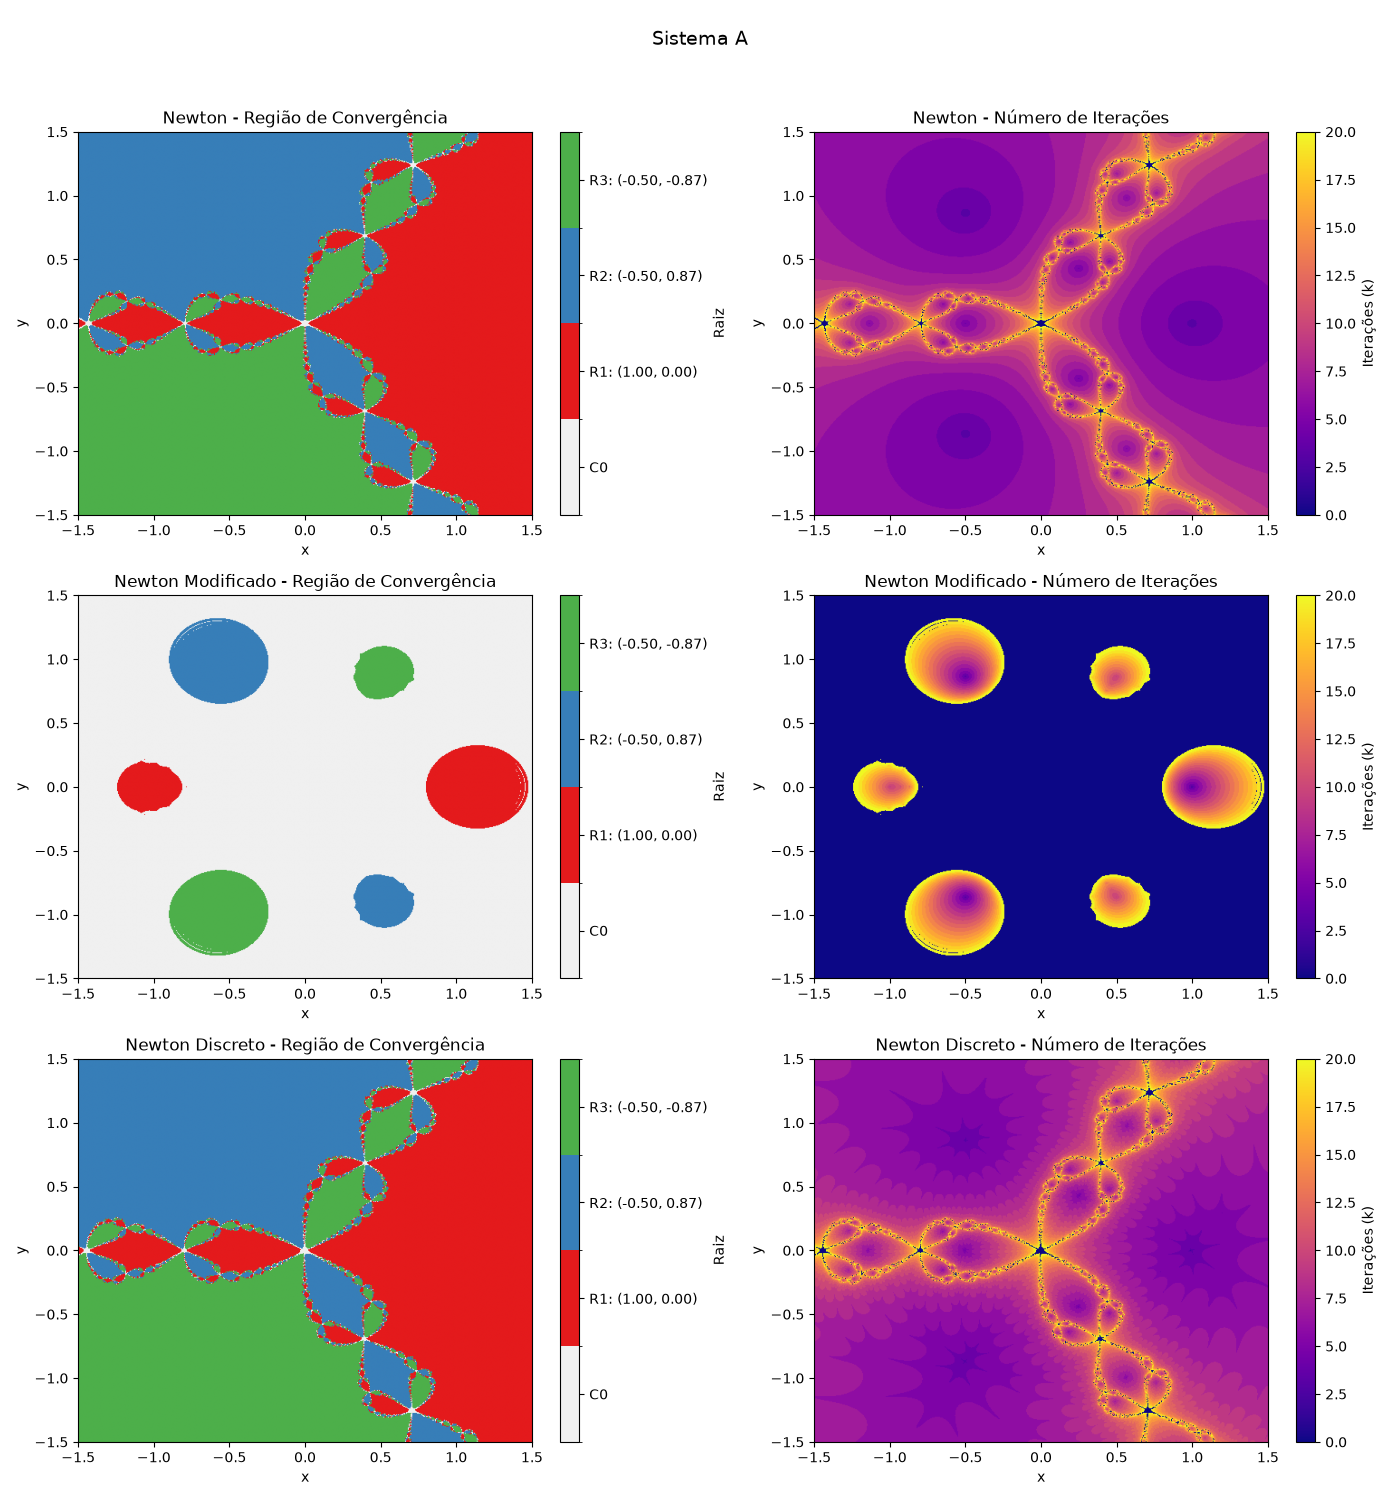
\includegraphics[width=0.6\textwidth]{sistemaA.png}
\caption{Gráficos das Convergências do Sistema $F_1(x,y)$}
\label{fig:rótulo}
\end{figure}

\begin{figure}[tphb]
\centering
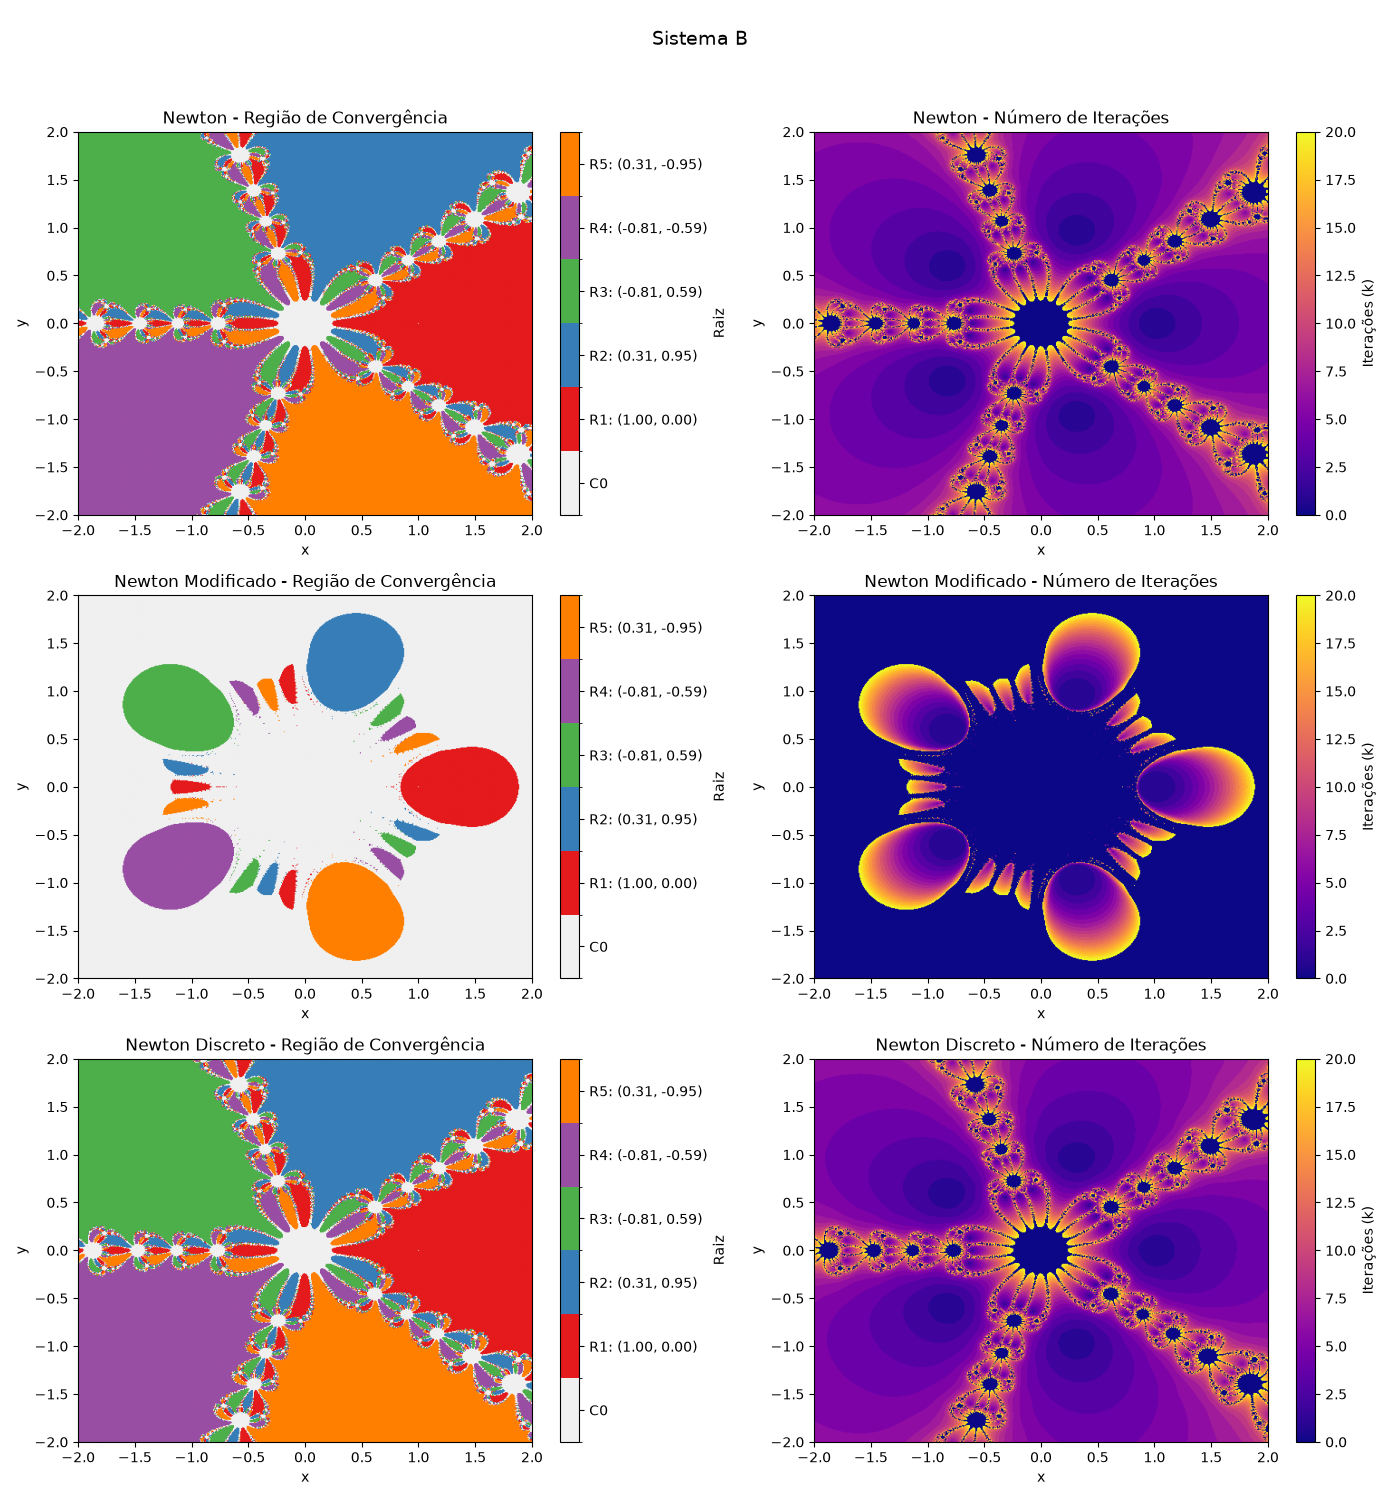
\includegraphics[width=0.6\textwidth]{sistemaB.png}
\caption{Gráficos das Convergências do Sistema $F_2(x,y)$}
\label{fig:rótulo}
\end{figure}
\end{document}